
\chapter{Test Cases \& Benchmarking Methodology}
\label{CHAPTER:BENCHMARKING}

This chapter first describes the test cases and shows how the data points are distributed for each case. Then, the benchmarking process and the tracked values are explained.

\section{Test Cases}
\label{SECTION:TESTCASES}

As in the SPH simulation, particles can be distributed within the domain in a variety of different ways. They can be arranged in many small clusters, or large groups. The cluster edges could be horizontal and vertical (i.e. parallel to the domain bounds) or at an angle. Depending on the contents of the simulation domain, there can be many points in the domain or only relatively few. The test cases are designed to cover these different varieties and allow for a comparison between them.

The test cases are differentiated by two important parameters, {\itshape fill} and {\itshape filltype}. The distribution and orientation of the points is determined by the fill type. Specifically, there are four different fill types: {\itshape full}, {\itshape clusters}, {\itshape corners}, and {\itshape diagonal}. Each are generated using the appropriate test case script as described in \ref{SECTION:TESTCASESCRIPTS}.

The second important parameter is the $fill$. This is defined as the fraction of actual points in the domain over the number of points in a fully-filled domain. The test case {\itshape full}, consisting of a fully-filled domain, has by definition a fill of $1.0$. For a domain size of $0.005$x$0.01$x$0.005$ and a particle spacing of $10^{-4}$, the {\itshape full} test case contains 250000 points distributed on a regular grid. The number of points in the other test cases is therefore always a fraction of 250000. 

\begin{figure}[h]
	\centering
	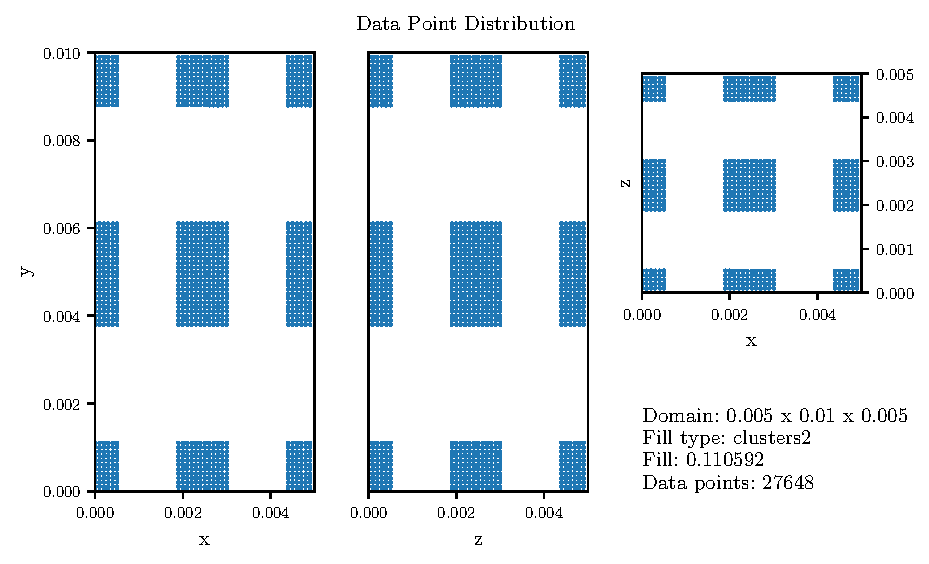
\includegraphics[]{figures/testcase_clusters2_11.pdf}
	\caption{Data points distribution for the clusters2 test case with 11\% fill.}
	\label{FIG:clusters2_11}
\end{figure}

The {\itshape clusters} test case is made up of rectangular, box-shaped clusters of points. Within the clusters, the points are distributed on a regular grid. The {\itshape clusters} cases are denoted {\itshape clusters}$N$, where the cluster size parameter $N$ specifies the number of clusters distributed throughout the space, i.e. a higher value of $N$ leads to more, but smaller clusters. The {\itshape clusters} test cases are examined for fill levels of 11\% and 51\% with varying cluster sizes. The cluster number parameter $N$ is set as an argument to the test case generation script. Exemplary {\itshape clusters} test cases for the same fill but different $N$ values can be see in the figures \ref{FIG:clusters2_11} and \ref{FIG:clusters6_11}. 

\begin{figure}[h]
	\centering
	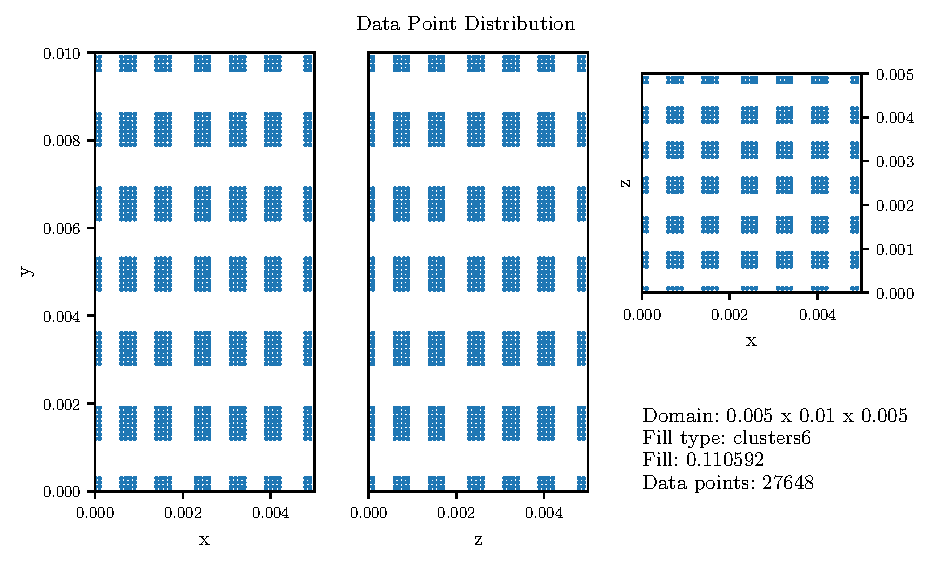
\includegraphics[]{figures/testcase_clusters6_11.pdf}
	\caption{Data points distribution for the clusters6 test case with 11\% fill.}
	\label{FIG:clusters6_11}
\end{figure}

The {\itshape corners} test case represent large groups of particles. The points are distributed regularly within two rectangular boxes extending from opposite corners of the domain towards the point in the center. This is visualized in Figure \ref{FIG:corners_11}. The maximum possible fill with this fill type is achieved when both boxes extend from their corners to the center. In this case two quarters of the domain are filled, leading to a fill of 50\%. The {\itshape corners} test case is examined for 2\%, 11\%, and 14\% fill.

\begin{figure}[h]
	\centering
	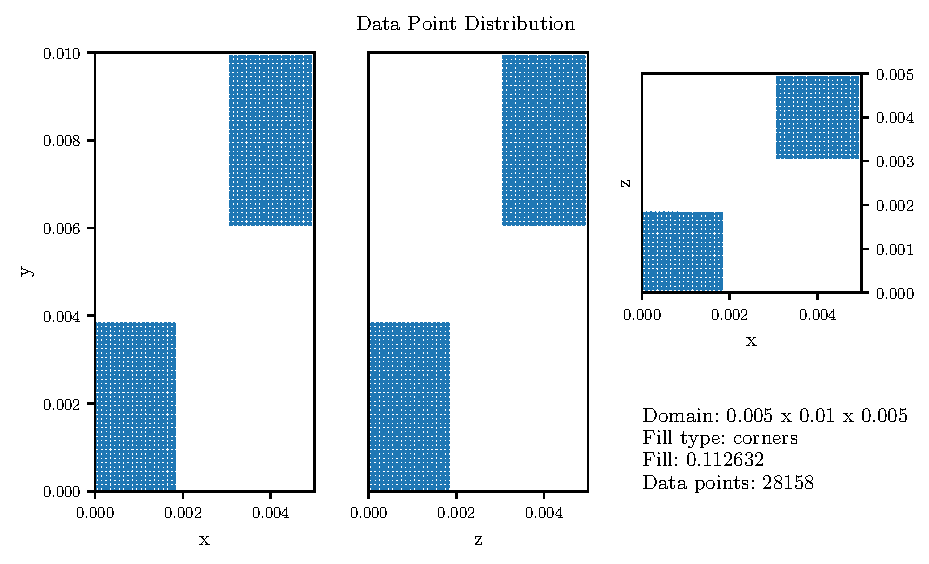
\includegraphics[]{figures/testcase_corners_11.pdf}
	\caption{Data points distribution for the corners test case with 11\% fill.}
	\label{FIG:corners_11}
\end{figure}

The {\itshape diagonals} test case is the only case in which the boundaries of the clusters are not parallel to the boundaries of the domain. The distribution is created by filling in the test domain from all eight corners up to a plane angled at 45 degrees from the domain boundaries. See Figure \ref{FIG:diagonals_11} for a 2D view of the {\itshape diagonals} test case with 11\% fill. This distribution is however best viewed in 3D using the {\itshape plot\_3d} script.

\begin{figure}[h]
	\centering
	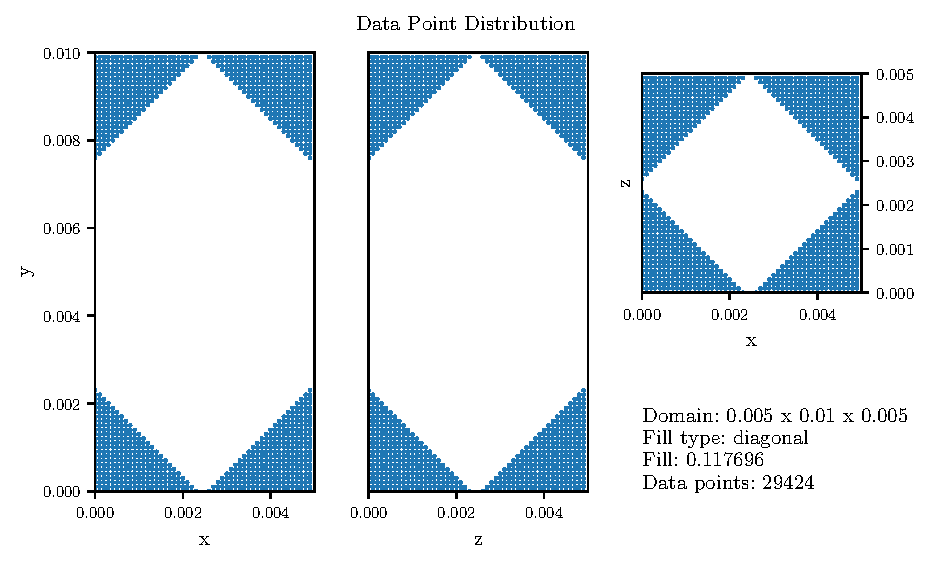
\includegraphics[]{figures/testcase_diagonal_11.pdf}
	\caption{Data points distribution for the diagonal test case.}
	\label{FIG:diagonals_11}
\end{figure}

\pagebreak

\section{Benchmarking}
\label{SECTION:BENCHMARKING}

\subsection{Tracked values}

In order to compare the performance of the search methods, two characteristic values are tracked. The first is the run time of the search: how much time it takes for the program to solve the frNN search problem and compile the results into a useful data format. This is achieved by using timers within the C++ implementation of the search methods. For all search methods, the total time, {\itshape ttotal}, is tracked. This total time does not include reading or writing data. For the ANN search, the time is additionally split up into the time spent determining the number of neighbors, {\itshape tksearch}, the time spent retrieving the neighbors from the kdtree structure, {\itshape tfrsearch}, and the time spent processing the interaction pair lists, {\itshape tprocessing}. The second tracked value is the memory use of the search method executable. This is measured by the {\itshape time} program, which outputs the maximum resident set size of the process. The resident set size is the space occupied by the process in the main memory (RAM).

\subsection{Benchmarking Process}

The benchmark is run via bash scripts for each search method, which define the test cases to run and also take care of tracking the memory use of the search processes. After the test case scripts and search method executables are copied to the test directory, the process as shown in Figure \ref{FIG:BENCHMARKING} is executed for each test case.

\begin{figure}[h]
	\centering
	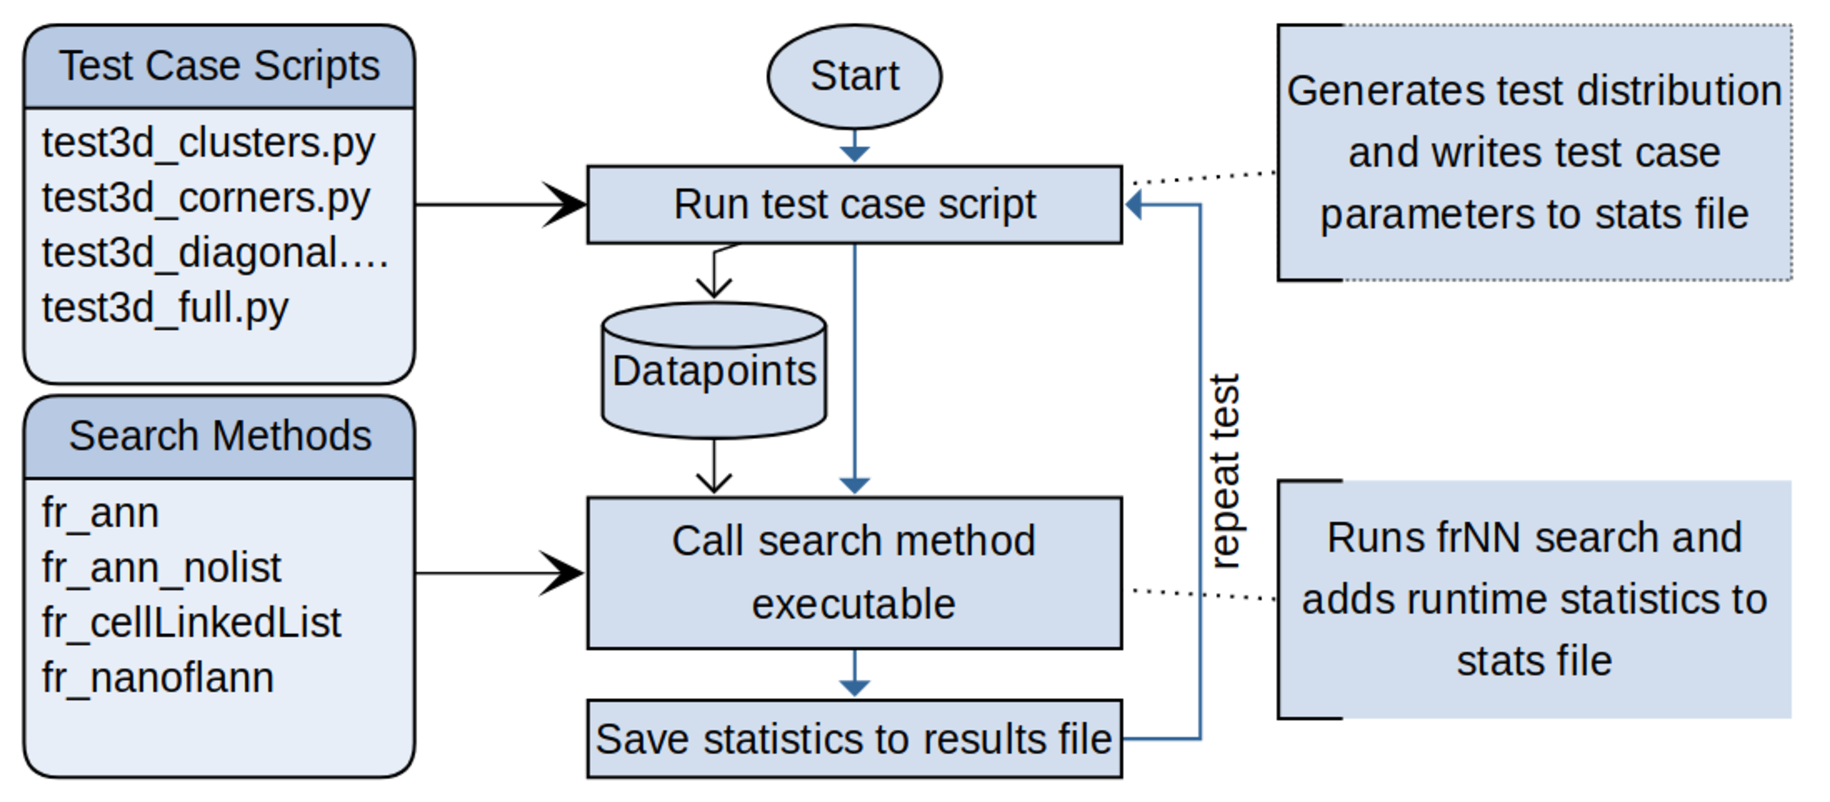
\includegraphics[width=0.75\textwidth]{figures/flowdiagram.pdf}
	\caption{The program flow for a test run with a certain test case and search method.}
	\label{FIG:BENCHMARKING}
\end{figure}

First, the test case script is called, which writes the data points and statistics file. The search method executable ist then executed using the {\itshape time} command to track the memory use of the process. The search method executable adds its own time results to the statistics file and once it is finished the memory use results are also added. This is repeated multiple times to get a statistically valid sample. The script then moves on to the next test case, repeating the described process.